\documentclass{beamer}

\useoutertheme{default}
\useoutertheme{hipinfolines}

\useinnertheme{rounded}

\newcommand{\todo}[1]{{\bf TODO:} {\em #1}}
% Meeting info:
\newcommand{\meeting}[0]{CMS Physics Analysis group meeting}
\newcommand{\meetingplace}[0]{}
\newcommand{\meetingdate}[0]{March 18th, 2008}
% End of meeting info

% Handout:
\usepackage{pgfpages}
%\pgfpagesuselayout{4 on 1}[a4paper,landscape,border shrink=5mm]

\title[P. Kaitaniemi (HIP): Distributed revision control...]{Distributed revision control with Git (Mar'08)} \author[\meeting, \meetingdate]{Pekka
Kaitaniemi \\ pekka.kaitaniemi@helsinki.fi} 

\institute[]{Helsinki
Institute of Physics} \date{\tiny \meetingdate \\ (Document built:
\today)}

\graphicspath{{.}{figures/}{images/}}

\begin{document}

\frame{\titlepage}

\section[Contents]{}
\frame{\tableofcontents}

\section{Revision control}

\subsection{History: from centralized to distributed}

\frame {
\frametitle{History of (open source) revision control}
The evolution of revision control:
\begin{itemize}
\item {\em Centralized lock-modify-unlock}
\begin{itemize}
\item RCS, SCCS
\item Tracked one file on one computer.
\end{itemize}
\item {\em Centralized copy-modify-merge}
\begin{itemize}
\item CVS (Concurrent Versions System), SVN (Subversion)
\item Track multiple files.
\item Multiple working copies and developers (possibly on different computers).
\item One central master repository on one computer.
\end{itemize}
\item {\em Distributed}
\begin{itemize}
\item Git, Bitkeeper (commercial) (also Mercurial, Bazaar-ng, Darcs)
\item Clone repositories: every developer has full revision history of
  the project.
\item No repository is inherently more important than any other
  repository.
\item The ``official version'' is a social notion, not a technical
  one!
\end{itemize}
\end{itemize}
}

\section{What is Git?}

\frame{
\frametitle{Git}

Revision control system originally developed by Linus Torvalds for use
in Linux kernel development.
\vskip0.5cm
Highly active project:
\begin{itemize}
\item Development started in 2005.
\item Became self-hosting Thu Apr 7 15:13:13 2005 (first commit).
\item 435 individual contributors and 13967 revisions during its
  lifetime.
\item Aims to make stable feature release every three months.
\end{itemize}
\vskip0.5cm
An implementation of a
\begin{itemize}
\item Distributed
\item High performance
\item Content tracker
\end{itemize}
}

\subsection{Distributed high performance content tracker}

\frame {
\frametitle{Distributed revision control}
\begin{itemize}
\item Every developer has a copy of the repository.
\item No single repository is inherently more important than any other
  repository.
\item Commit locally, push/pull changes between repositories and
  developers.
\item Merging development histories between developers is extremely
  important!
\end{itemize}

Benefits:
\begin{itemize}
\item Empowers the developers and users: everyone has full access.
\item No need to maintain a server, grant/revoke commit privs,
  i.e. low management overhead.
\item No single point of control, no single point of failure.
\item Network of trust: Developers can choose whom they trust (from
  whom they accept code from).
\item Full offline access to revision control machinery.
\end{itemize}
}

\frame {
\frametitle{High performance}

High performance was a design requirement from the beginning.
\begin{itemize}
\item Mostly faster than any other revision control tool.
\item Implemented in bare C.
\item Local operations: no networking overhead. Supports committing
  early and often, using diffs, logs and all the revision control
  machinery all the time.
\item Fast branching and merging.
\item Highly compressed data storage.
\item Scalability behaviour: optimized for project revisions instead
  of single file versioning (example: log (diff) of the whole project
  is generated faster than log (diff) of one file).
\end{itemize}

Performance is not only about doing the same thing faster. It allows
users to work in a completely different manner!

}

\frame {
\frametitle{Content tracker}

It's not about ``file revisions''...
\begin{itemize}
\item What combination of file revisions is needed for a certain
  product version? In CVS tagging is the only way to overcome this
  limitation...
\item Thinking in terms of individual file revisions is not
  sufficient.
\item The project revisions are much more important!
\end{itemize}

Git is not interested in files at all:
\begin{itemize}
\item It tracks content changes.
\item Git can identify that a code fragment (e.g. a function) was
  moved from one file to another!
\item File renames are a special case of content tracking.
\end{itemize}
}

\section{Basic Git usage}

\subsection{Basic operations}

\frame {
\frametitle{Basic operations}
\begin{minipage}{1.0\linewidth}
\begin{minipage}{0.5\linewidth}
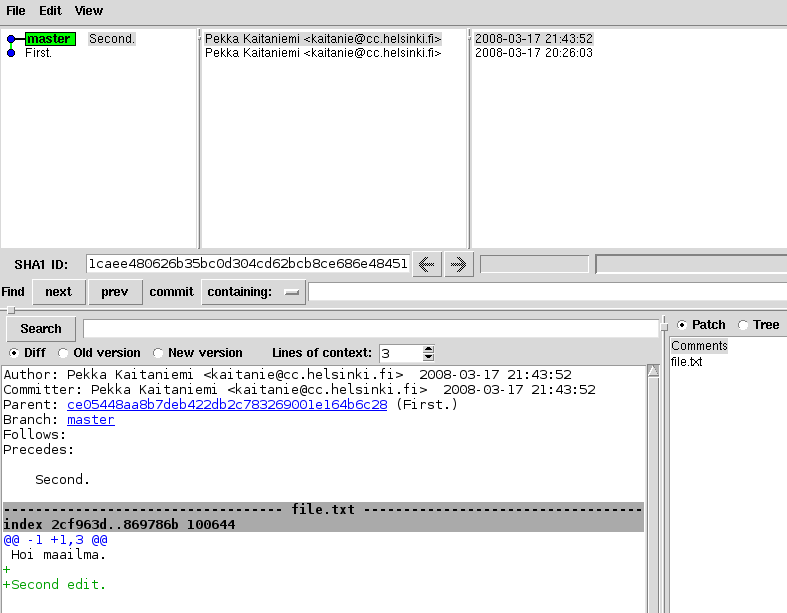
\includegraphics[scale=0.30]{images/first.png}
\end{minipage}
\begin{minipage}{0.5\linewidth}
Creating a new repository:
\begin{itemize}
\item {\tt mkdir test ; cd test}
\item {\tt git init}
\end{itemize}
Making commits:
\begin{itemize}
\item {\tt edit file.txt}
\item {\tt git add file.txt}
\item {\tt git commit -m "First."}
\item {\tt edit file.txt}
\item {\tt git add file.txt}
\item {\tt git commit -m "Second."}
\end{itemize}
Visualization tool (see Fig):
\begin{itemize}
\item {\tt gitk}
\end{itemize}
\end{minipage}
\end{minipage}
}

\subsection{Branching}

\frame{
\frametitle{Branching and switching branches}
Creating a new branch:
\begin{minipage}{1.0\linewidth}
\begin{minipage}{0.5\linewidth}
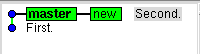
\includegraphics[scale=1.00]{new-branch.png}
\end{minipage}
\begin{minipage}{0.5\linewidth}
\begin{itemize}
\item {\tt git branch new}
\end{itemize}
\end{minipage}
\end{minipage}
\begin{minipage}{1.0\linewidth}
\begin{minipage}{0.5\linewidth}
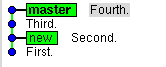
\includegraphics[scale=1.00]{branches.png}
\end{minipage}
\begin{minipage}{0.5\linewidth}
\begin{itemize}
\item {\tt edit file.txt}
\item {\tt git commit -a -m "Third."}
\item {\tt edit file.txt}
\item {\tt git commit -a -m "Fourth."}
\end{itemize}
\end{minipage}
\end{minipage}
Committing changes to a branch:
\begin{minipage}{1.0\linewidth}
\begin{minipage}{0.5\linewidth}
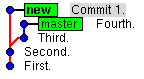
\includegraphics[scale=1.00]{branch-commit.png}
\end{minipage}
\begin{minipage}{0.5\linewidth}
\begin{itemize}
\item {\tt git checkout new}
\item {\tt edit file.txt}
\item {\tt git commit -a -m "Commit 1."}
\end{itemize}
\end{minipage}
\end{minipage}
}

\subsection{Merging}

\frame {
\frametitle{Merging branches}
Merge branch ``next'' to ``master'':
\begin{minipage}{1.0\linewidth}
\begin{minipage}{0.5\linewidth}
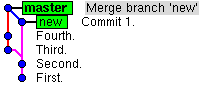
\includegraphics[scale=1.00]{merge.png}
\end{minipage}
\begin{minipage}{0.5\linewidth}
\begin{itemize}
\item {\tt git checkout master}
\item {\tt git merge new}
\end{itemize}
\end{minipage}
\end{minipage}
\vskip0.3cm

The benefits of branching and merging:
\begin{itemize}
\item Separate development and stable lines.
\item Topic branches: develop a feature in a branch, test it and merge
  to mainline when it is stable enough.
\item Branches encourage ``speculative'' development, i.e. asking the
  question ``What if?''
\item In a distributed system every developer is working on a separate
  branch.
\end{itemize}
}

\section{Collaborative development}

\subsection{Publishing a repository on the web}

\frame {
\frametitle{Publishing a repository on the web}

Prepare an empty public repository as {\tt user} on machine {\tt
example.org}:
\begin{itemize}
\item {\tt cd \$HOME/public\_html}  (at CERN: {\tt cd \$HOME/public/html})
\item {\tt mkdir myproject.git; cd myproject.git}
\item {\tt git --bare init}
\item {\tt chmod a+x hooks/post-update}
\item {\tt git update-server-info}
\end{itemize}
\vskip0.5cm
Push your work to that repository:
\begin{itemize}
\item {\tt git remote add public ssh://user@example.org/path/to/myproject.git}
\item {\tt git push public refs/heads/master:refs/heads/master}
\end{itemize}
}

\subsection{Push/Pull model}
\frame {
\frametitle{Pushing and pulling changes}
Each developer has his/her own repository.
\vskip0.3cm
\begin{itemize}
\item Push = Put changes to a remote repository.
\item Pull = {\em fetch} changes from remote repository and {\em
  merge} them.
\end{itemize}
\vskip0.3cm
Sharing changes between developers:
\begin{itemize}
\item Maintainer pulls from developers.
\begin{itemize}
\item Probably the simplest distributed workflow.
\item Clearly defined ``official version''.
\end{itemize}
\item Everyone pulls from everyone else.
\begin{itemize}
\item Mainly useful for few developers.
\item Probably confusing for new users.
\end{itemize}
\item All developers push to a shared repository (CVS like workflow).
\begin{itemize}
\item Does not take advantage of distribution. Everyone working in the
  same sandbox. Not really recommended.
\end{itemize}
\end{itemize}
}

\section{Conclusions}

\frame {
\frametitle{Summary and conclusions}

}

\end{document}
